\documentclass[dvipdfmx]{jsarticle}
% for png
\usepackage[dvipdfmx]{graphicx}
% for positioning
\usepackage{here}
% color
\usepackage[dvipdfmx]{graphics, color}
% hyperlink用package
\usepackage[dvipdfmx]{hyperref}
\usepackage{pxjahyper}
\hypersetup{
    bookmarksnumbered=true,%
    bookmarksopen=true,%
    colorlinks=true,%
    linkcolor=blue,
    citecolor=red,
}
% for source code
\usepackage{listings,jvlisting}
\lstset{
    language=c, % default language
    numbers=none, % line number sample)left, right, none
    numbersep=10pt, % space between linenumber to source code
    tabsize=2,
    breaklines=false, % breaking line, if src is too long
    breakindent=10pt, % indent size
    frame=lines, % frame sample)single, topline, shadowbox
    framesep=5pt, % space between frame to source code
}

\begin{document}

\title{LaTeX環境構築}
\author{黒馬裕貴}
\maketitle

\section{はじめに}

この文書は,WindowsでのTexのインストールから,
VSCodeとその拡張機能LaTeX Workshopを用いた環境構築のやり方をまとめます。

\section{TeXのインストール}

この文書ではネットワークインストーラーを利用してTeX Liveをインストールします。

\subsection{ネットワークインストーラーのダウンロード}

\href{https://www.tug.org/texlive/acquire-netinstall.html}{Installing TeX Live over the Internet}から
install-tl-windows.exeをダウンロードします。(もしリンク切れを起こしている場合は、\href{https://texwiki.texjp.org/}{TeX Wiki}から
ダウンロードページへ移動してください。)

\href{https://www.tug.org/texlive/acquire-netinstall.html}{Installing TeX Live over the Internet}
を開くと図1のようなWebページが表示されます。図1上部のオレンジ色の枠のいずれかにあるリンクをクリックしてもらうと、
図1下部の赤色の枠のようなものが表示されるのでクリックしてください。

\begin{figure}[H]
    \begin{center}
    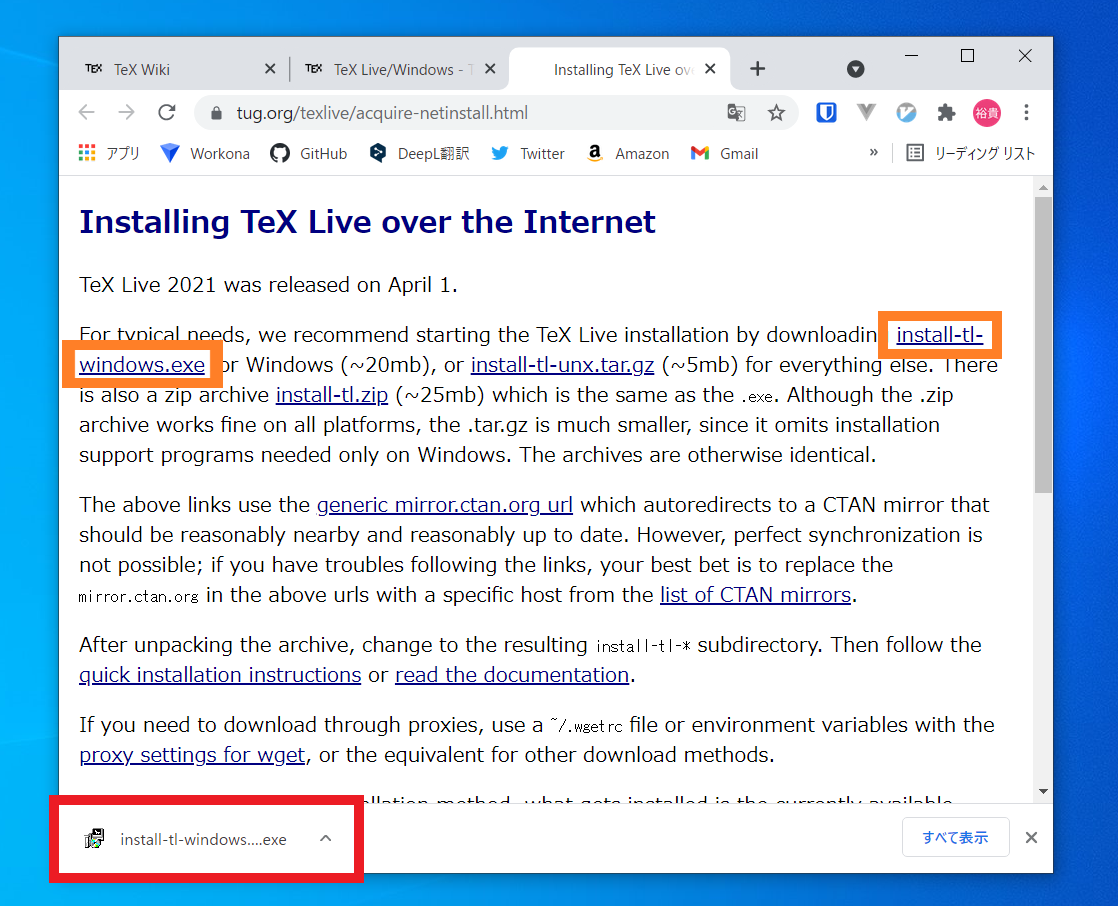
\includegraphics[width=5cm]{images/InstallingTexLiveOverTheInterner.png}
    \caption{Installing Tex Live over the internet}
    \end{center}
\end{figure}

クリックするとWindowsDefenderが起動してPCが保護されるので、
図2の赤い枠の詳細情報をクリックして、
図3を表示したのち、下部の赤枠から実行をクリックし、
インストールを開始してください。
以上でネットワークインストーラーのダウンロードは終了です。

\begin{figure}[H]
    \begin{minipage}[b]{0.45\linewidth}
        \centering
        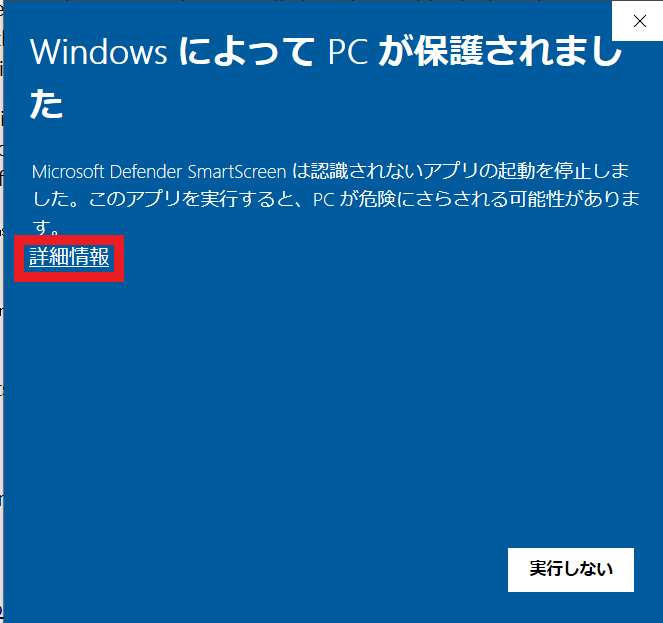
\includegraphics[width=5cm]{images/WindowsDefender1.png}
        \caption{WindowsDefender1}
    \end{minipage}
    \begin{minipage}[b]{0.45\linewidth}
        \centering
        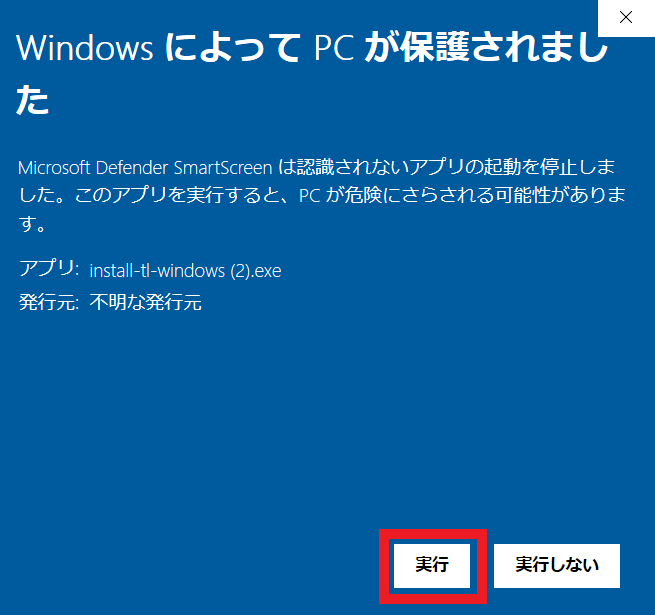
\includegraphics[width=5cm]{images/WindowsDefender2.png}
        \caption{WindowsDefender2}
    \end{minipage}
\end{figure}

\subsection{TeX Live Installerのインストール}

ネットワークインストーラーのダウンロードが完了すると図4が表示されます。
そうしたら、オレンジ線のようにInstallが選択されていることを確認し、
選択されていれば、下部の赤枠のNextをクリックしてください。
Nextをクリックすると図5のような画面がでるとおもうので、
画面下部の赤枠のInstallをクリックして、インストールを開始します。
図6のような画面になったとき、インストールが完了します。

\begin{figure}[H]
    \begin{minipage}[b]{0.33\linewidth}
        \centering
        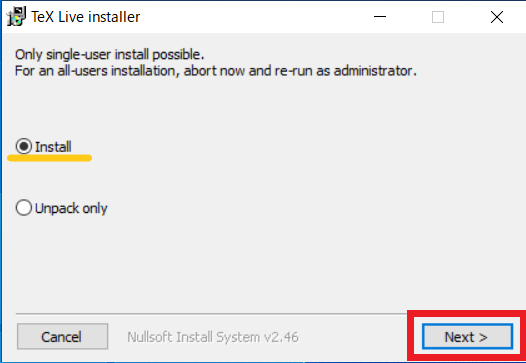
\includegraphics[width=5cm]{images/TeXLiveInstaller1.png}
        \caption{TexLiveInstaller1}
    \end{minipage}
    \begin{minipage}[b]{0.33\linewidth}
        \centering
        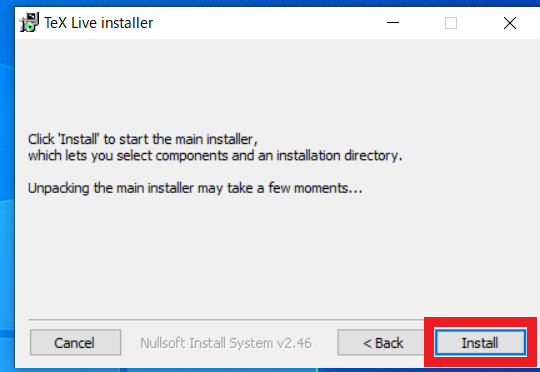
\includegraphics[width=5cm]{images/TeXLiveInstaller2.png}
        \caption{TexLiveInstaller2}
    \end{minipage}
    \begin{minipage}[b]{0.33\linewidth}
        \centering
        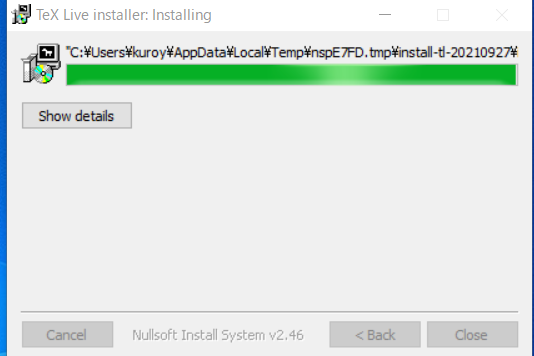
\includegraphics[width=5cm]{images/TeXLiveInstaller3.png}
        \caption{TexLiveInstaller3}
    \end{minipage}
\end{figure}

\subsection{TeX Liveのインストール}
お待たせしました。これからTeX Liveのインストールを行います。
TeX Live Installerがインストールされると図7のような画面が表示されます。
デフォルトで設定されているフルインストールをすると2時間近くかかってしまうので、
図7の下部の赤枠にある「高度な設定」をクリックして、
カスタムインストールをおこないます。

\begin{figure}[H]
        \centering
        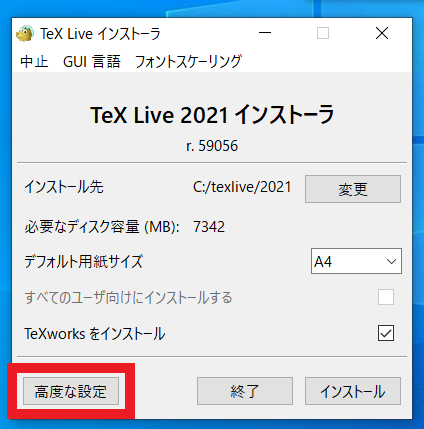
\includegraphics[width=5cm]{images/TeXLive2021_1.png}
        \caption{インストール開始画面}
\end{figure}

図8がカスタムインストール画面になります。
デフォルトではオレンジ線の部分のように「fullスキーム」が設定されています。
変更するために、図8の下部の赤枠の変更ボタンをクリックしてください。
図9のようなスキーム選択画面が表示されます。
「basicスキーム」をクリックしたのち、
図9の下部の赤枠のOKボタンをクリックしてください。
選択が成功していると、図10のように「besicスキーム」が表示されます。

\begin{figure}[H]
    \begin{minipage}[b]{0.33\linewidth}
        \centering
        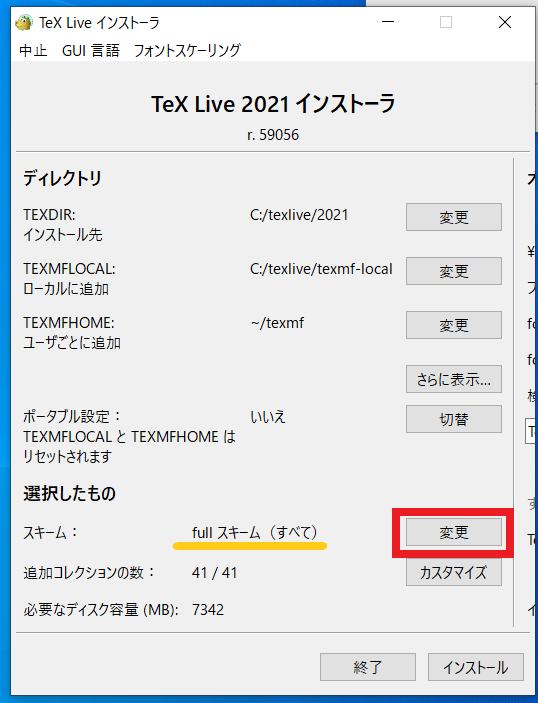
\includegraphics[width=5cm]{images/TeXLive2021_2.png}
        \caption{カスタムインストール画面}
    \end{minipage}
    \begin{minipage}[b]{0.33\linewidth}
        \centering
        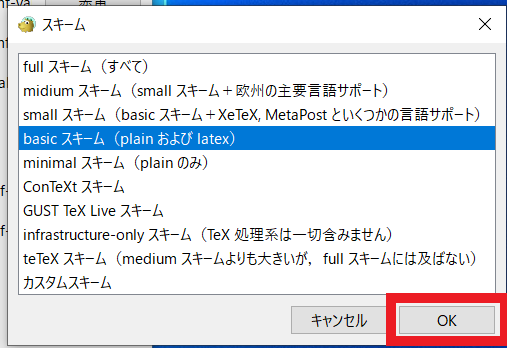
\includegraphics[width=5cm]{images/TeXLive2021_3.png}
        \caption{スキーム選択画面}
    \end{minipage}
    \begin{minipage}[b]{0.33\linewidth}
        \centering
        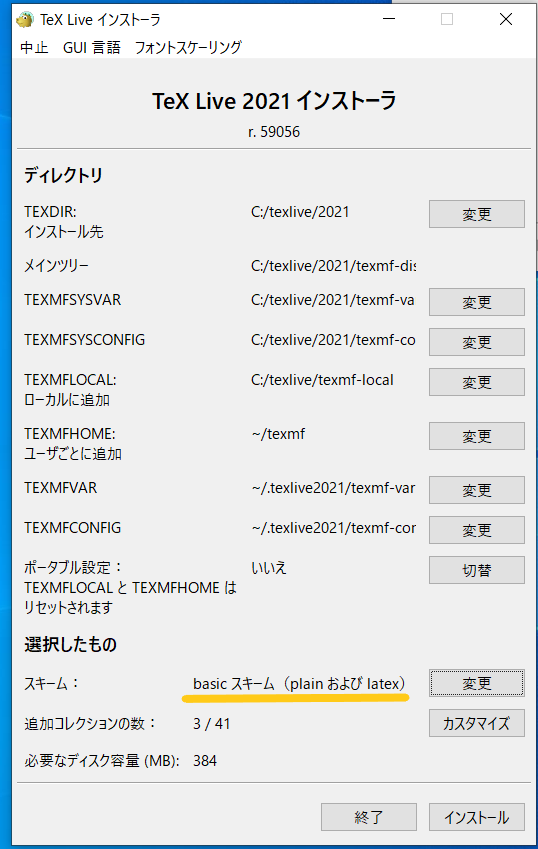
\includegraphics[width=5cm]{images/TeXLive2021_4.png}
        \caption{スキーム選択後画面}
    \end{minipage}
\end{figure}

% 続きはここから
% 画像の貼り付けから再始動
次に「basicスキーム」では不足してしまっている必要なパッケージをインストールします。
図11下部の赤枠のカスタマイズボタンをクリックして、
コレクション選択画面に移動してください。
図12がコレクション選択画面になります。

下記のコレクションをクリックし、図12と同様になったのち、
図12下部の赤枠のOKボタンをクリックしてください


\begin{itemize}
    \item 言語
    \begin{itemize}
        \item 日本語
    \end{itemize}
    \item ほかのコレクション
    \begin{itemize}
        \item LaTeX 推奨パッケージ
        \item 数学,自然科学,計算機科学パッケージ
        \item 画像と図表
    \end{itemize}
\end{itemize}

図12のOKボタンをクリックするとカスタムインストール画面に戻ります。
図13と同様になっていることを確認してください。
確認の後、図13下部の赤枠のインストールボタンをクリックしてください。

\begin{figure}[H]
    \begin{minipage}[b]{0.33\linewidth}
        \centering
        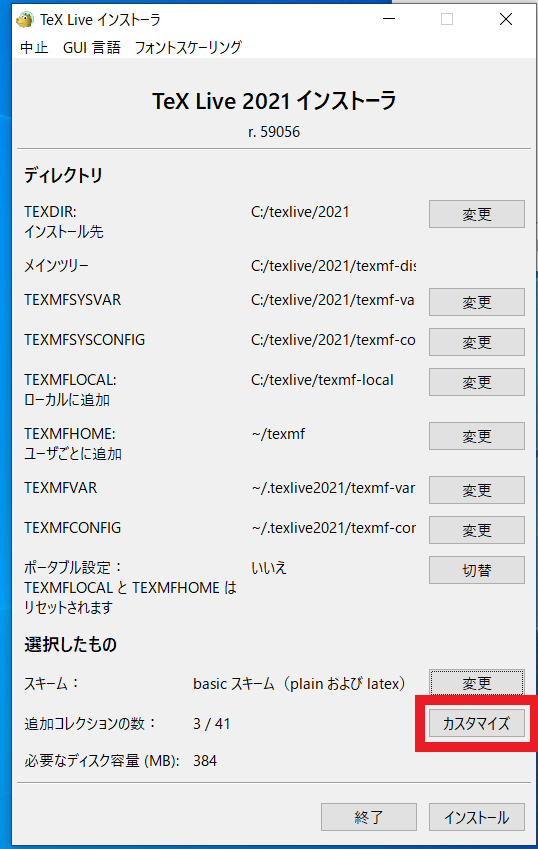
\includegraphics[width=5cm]{images/TeXLive2021_5.png}
        \caption{カスタムインストール画面2}
    \end{minipage}
    \begin{minipage}[b]{0.33\linewidth}
        \centering
        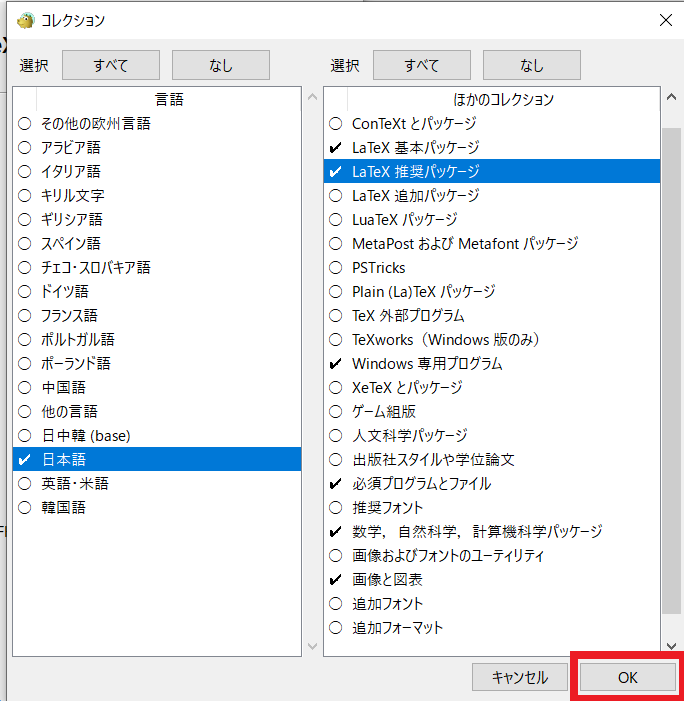
\includegraphics[width=5cm]{images/TeXLive2021_6.png}
        \caption{コレクション選択画面}
    \end{minipage}
    \begin{minipage}[b]{0.33\linewidth}
        \centering
        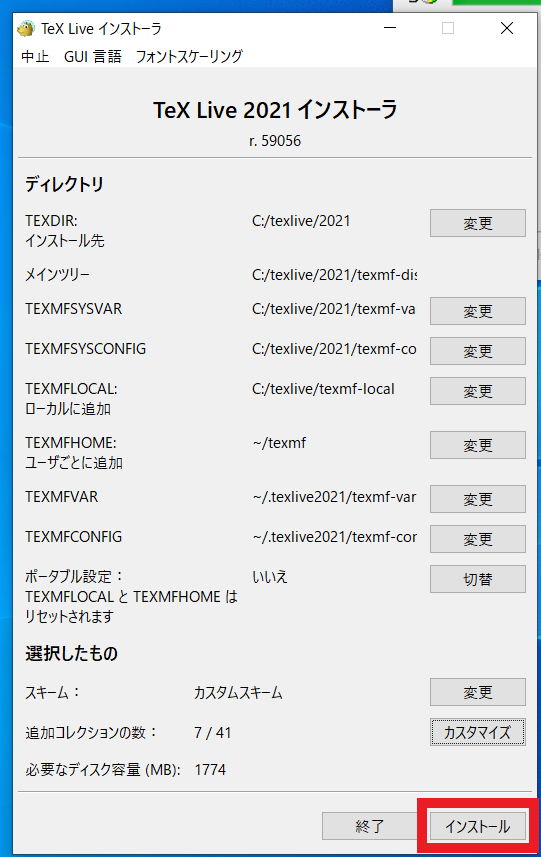
\includegraphics[width=5cm]{images/TeXLive2021_7.png}
        \caption{カスタムインストール画面3}
    \end{minipage}
\end{figure}

あとはインストールが完了するまで待機してください。
図14のような画面になったとき、インストールが完了しています。
閉じるボタンを押して、インストーラーを終了してください。
お疲れ様でした。

\begin{figure}[H]
    \centering
    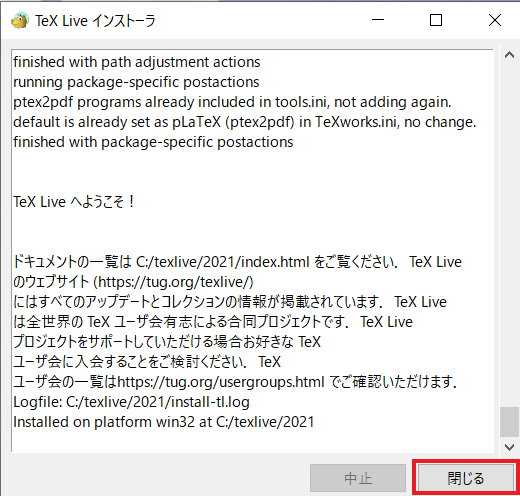
\includegraphics[width=5cm]{images/TeXLive2021_8.png}
    \caption{インストール完了画面}
\end{figure}


\section{VSCodeのインストール}

\href{https://code.visualstudio.com/}{Visual Studio Code}のホームページからインストールを行います。
赤色の文字列のリンクから飛ぶか、URL(\href{https://code.visualstudio.com/}{https://code.visualstudio.com/})からホームページへ移動してください。

ホームページにたどり着いたら図15赤枠の『Download for Windows』をクリックしてください。
クリックすると図16のようにページが遷移するので、図16左下の赤枠をクリックして、インストーラーのダウンロードを開始してください。

\begin{figure}[H]
    \begin{minipage}[b]{0.495\linewidth}
        \centering
        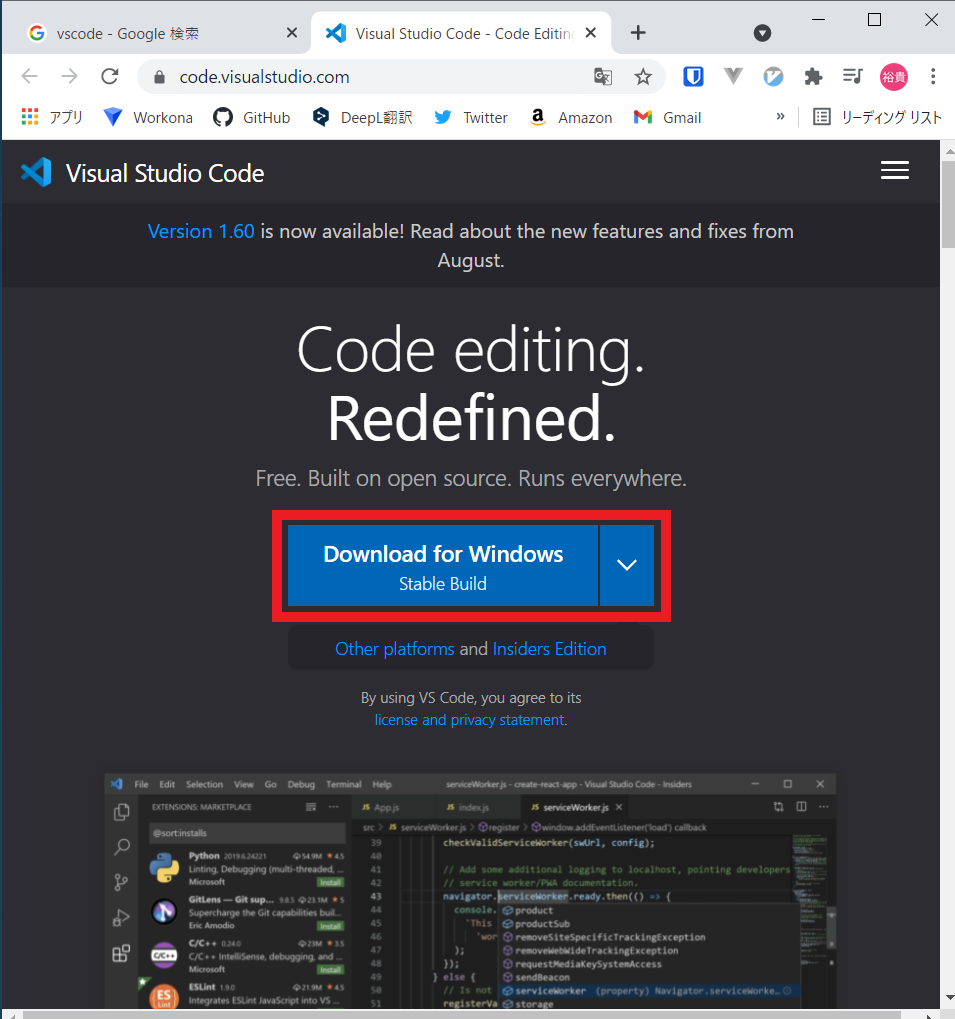
\includegraphics[width=5cm]{images/VSCodeInstall1.png}
        \caption{VScode ホームページ}
    \end{minipage}
    \begin{minipage}[b]{0.495\linewidth}
        \centering
        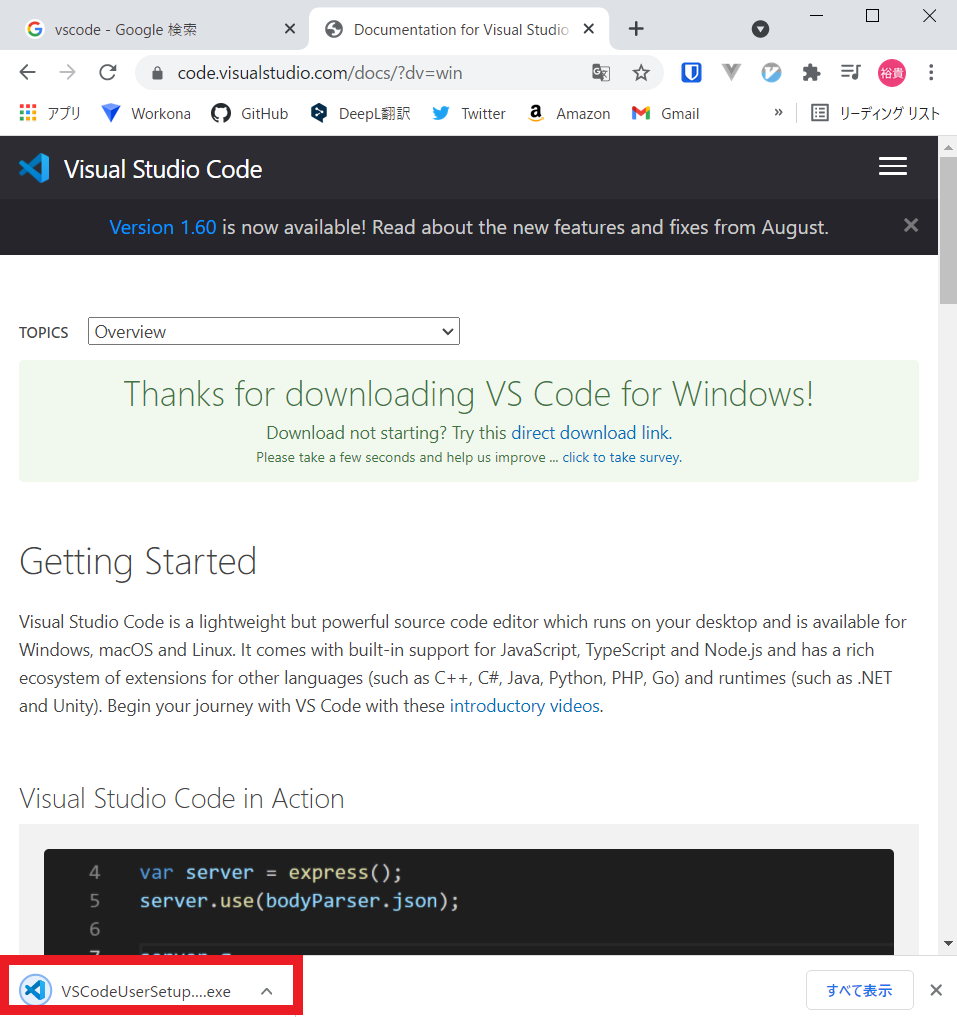
\includegraphics[width=5cm]{images/VSCodeInstall2.png}
        \caption{インストーラーのダウンロード開始画面}
    \end{minipage}
\end{figure}

インストーラーが起動されると図17のような画面が表示されます。
図17のオレンジ枠のように『同意する』を選択した後、赤枠の『次へ』をクリックしてください。
図18のようにインストール先を指定する画面が表示されます。
指定がなければ、赤枠の『次へ』をクリックしてください。
図19が表示されます。
図18と同様、指定がなければ赤枠の『次へ』をクリックしてください。

\begin{figure}[H]
    \begin{minipage}[b]{0.33\linewidth}
        \centering
        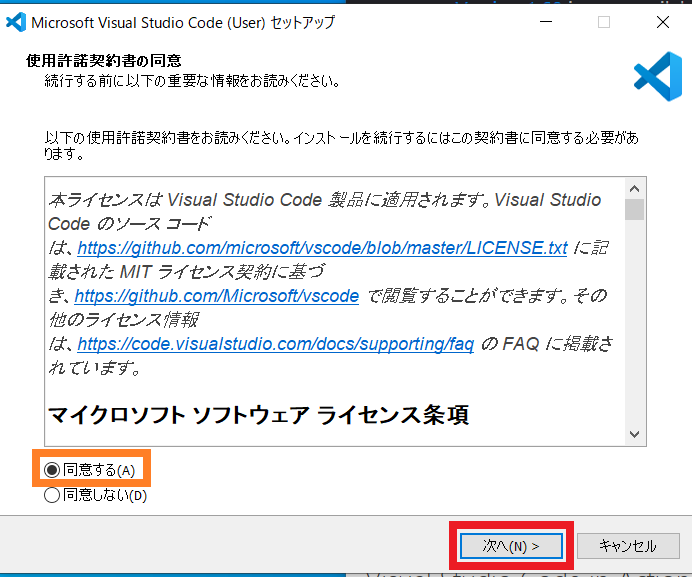
\includegraphics[width=5cm]{images/VSCodeInstaller1.png}
        \caption{インストール同意画面}
    \end{minipage}
    \begin{minipage}[b]{0.33\linewidth}
        \centering
        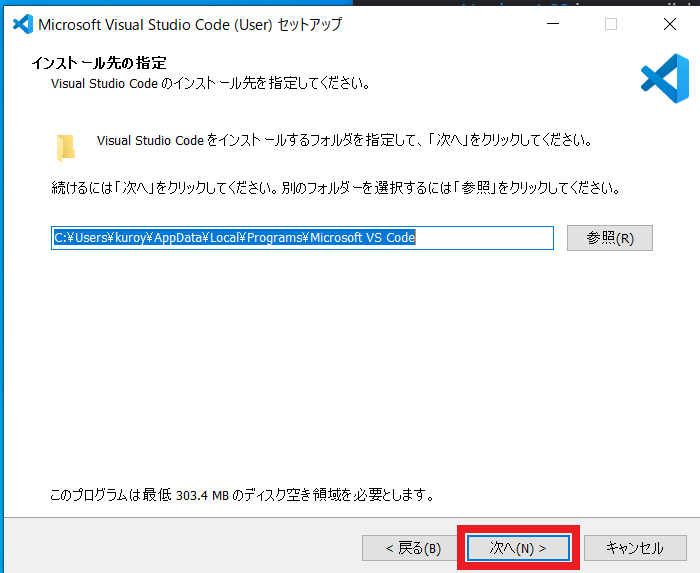
\includegraphics[width=5cm]{images/VSCodeInstaller2.png}
        \caption{インストール先指定画面}
    \end{minipage}
    \begin{minipage}[b]{0.33\linewidth}
        \centering
        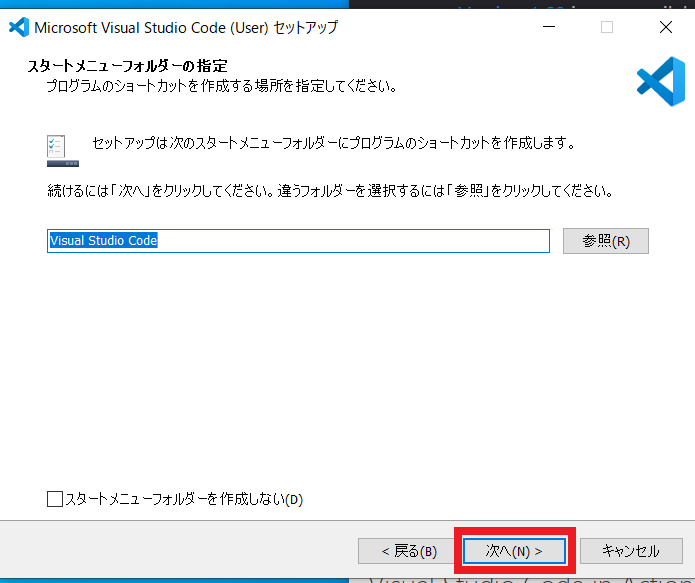
\includegraphics[width=5cm]{images/VSCodeInstaller3.png}
        \caption{ショートカット作成画面}
    \end{minipage}
\end{figure}

図20が表示されたら、オレンジ枠の『デスクトップ上にアイコンを作成する』をクリックしたのち、
赤枠の『次へ』をクリックしてください。
図21が表示されたら、赤枠の『インストール』をクリックしてVSCodeのインストールを開始してください。
図22が表示されたら、インストールが完了しています。
赤枠の『完了』をクリックしてください。
以上でVSCodeのインストールは終了です。

\begin{figure}[H]
    \begin{minipage}[b]{0.33\linewidth}
        \centering
        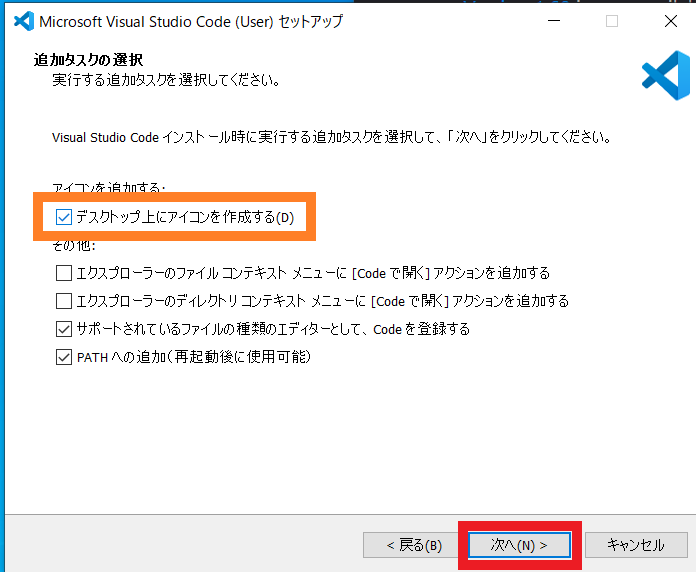
\includegraphics[width=5cm]{images/VSCodeInstaller4.png}
        \caption{追加タスク選択画面}
    \end{minipage}
    \begin{minipage}[b]{0.33\linewidth}
        \centering
        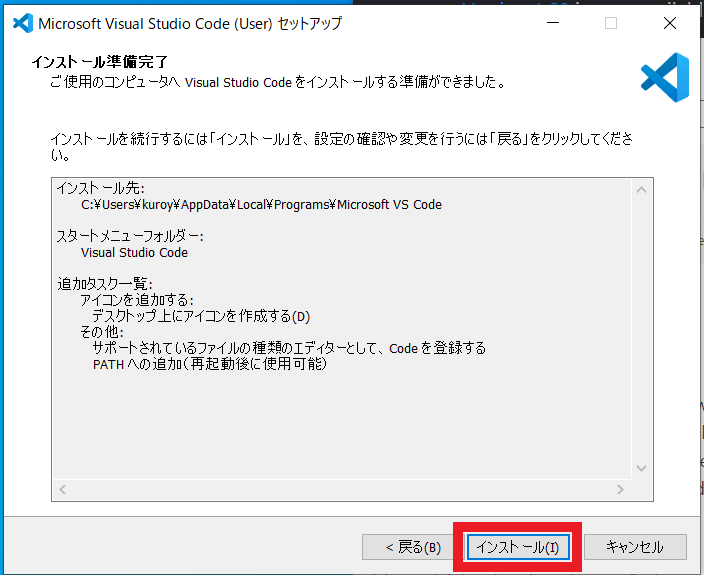
\includegraphics[width=5cm]{images/VSCodeInstaller5.png}
        \caption{インストール開始画面}
    \end{minipage}
    \begin{minipage}[b]{0.33\linewidth}
        \centering
        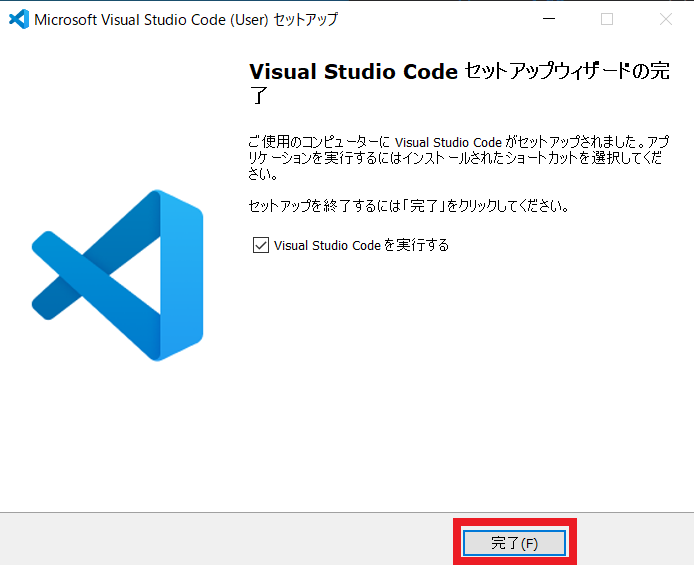
\includegraphics[width=5cm]{images/VSCodeInstaller6.png}
        \caption{インストール完了画面}
    \end{minipage}
\end{figure}

\section{VSCodeのセットアップ}

\subsection{VSCodeのテーマ設定}

図22で『完了』をクリックしていれば、VSCodeが起動して図23のような画面が表示されていると思います。(2021年10月時点)
利用するテーマに指定がなければ、図23の赤枠のように『Dark』をクリックしてください。
図24のように画面が切り替わればテーマの設定は終了です。

\begin{figure}[H]
    \begin{minipage}[b]{0.45\linewidth}
        \centering
        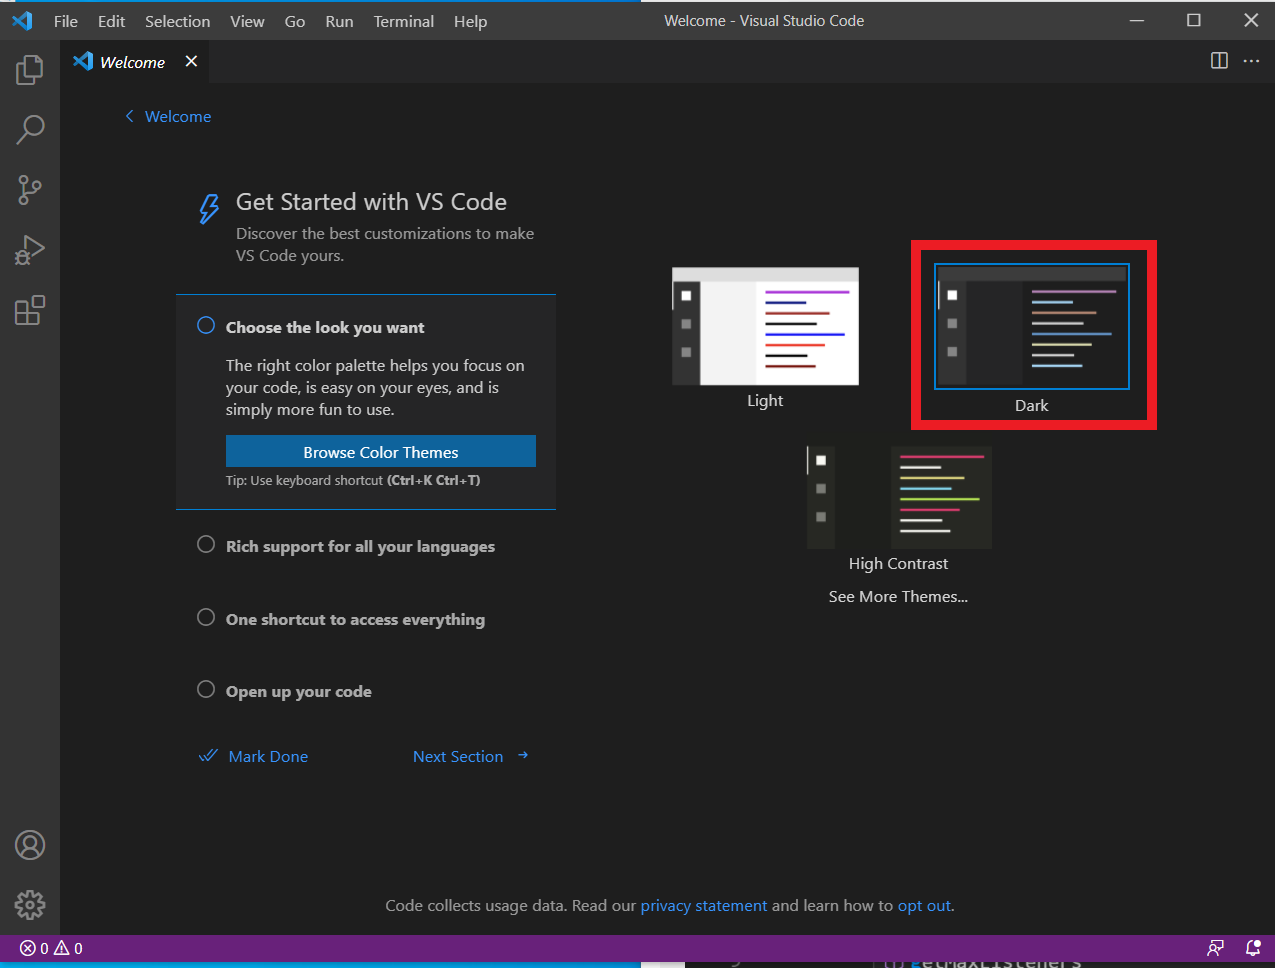
\includegraphics[width=5cm]{images/VSCode1.png}
        \caption{VSCode初期画面1}
    \end{minipage}
    \begin{minipage}[b]{0.45\linewidth}
        \centering
        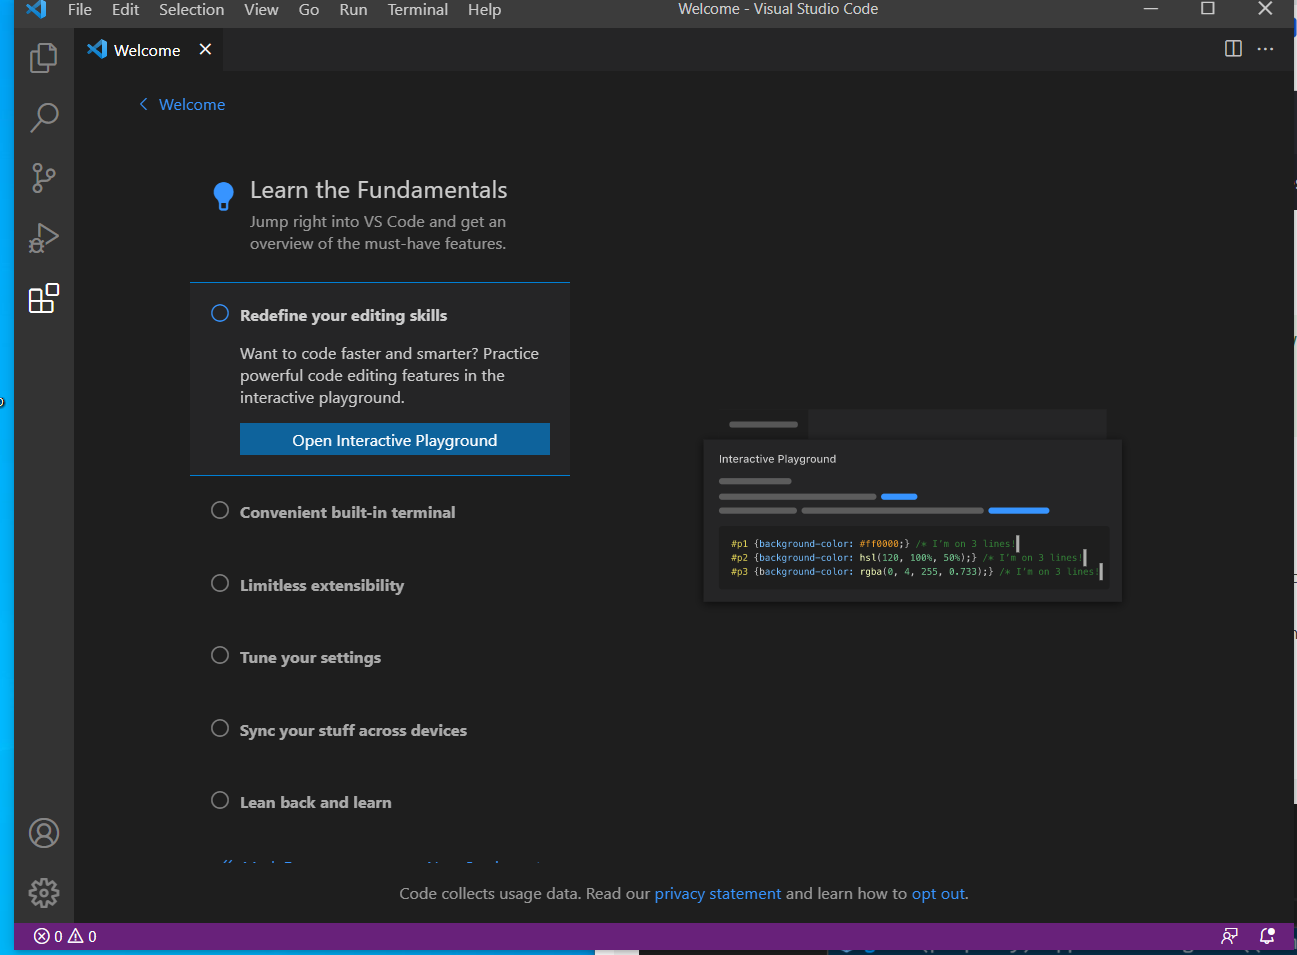
\includegraphics[width=5cm]{images/VSCode2.png}
        \caption{VSCode初期画面2}
    \end{minipage}
\end{figure}

\subsection{VSCodeの日本語化}

初期設定のVSCodeは英語で設定されています。日本語化していきましょう。
図25の赤枠にある四角形が4つあるアイコンをクリックしてください。
図26のオレンジ枠にある検索枠が表示されたら『japan』と入力してください。
赤枠のような地球儀のアイコンをクリックしてください。
『Japanese Language Pack for Visual Studio Code』が表示されます。
その後は、緑枠の位置にある『install』をクリックしてください。

\begin{figure}[H]
    \begin{minipage}[b]{0.45\linewidth}
        \centering
        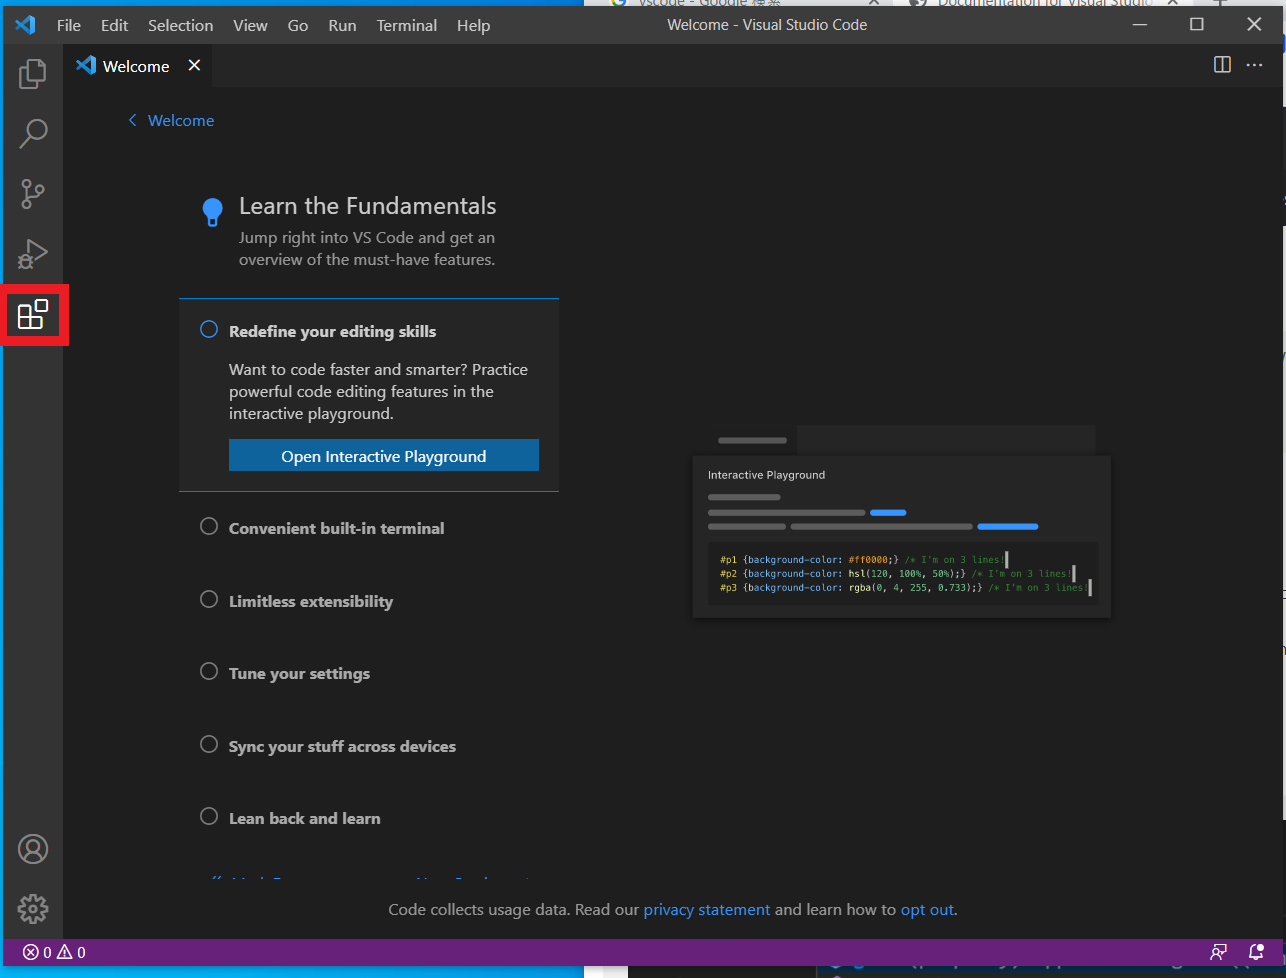
\includegraphics[width=5cm]{images/VSCodeExtension1.png}
        \caption{VSCode初期画面}
    \end{minipage}
    \begin{minipage}[b]{0.45\linewidth}
        \centering
        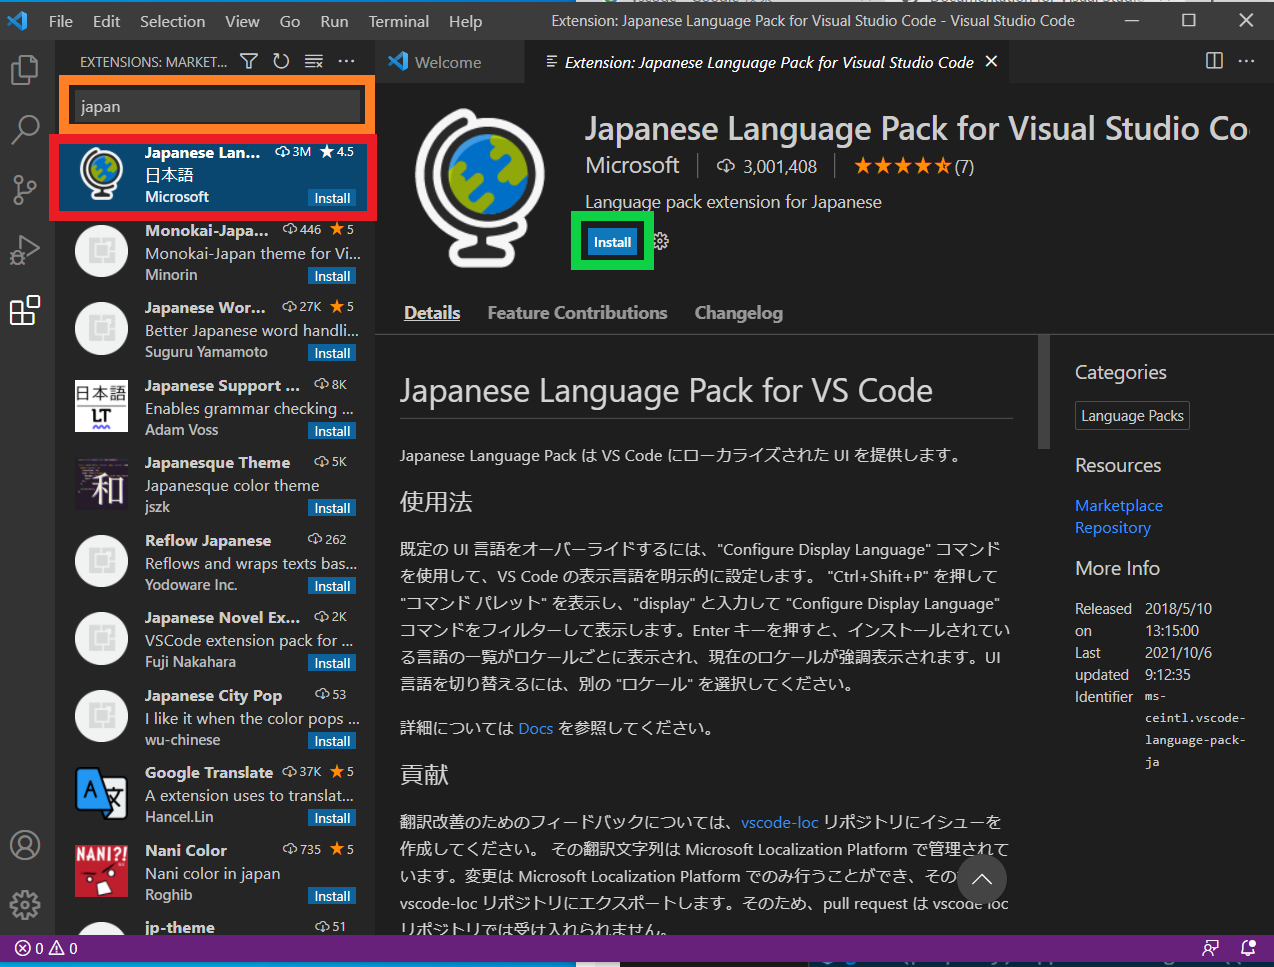
\includegraphics[width=5cm]{images/VSCodeExtension2.png}
        \caption{日本語パッケージ選択画面}
    \end{minipage}
\end{figure}

日本語パッケージのインストールが完了すると、図27のような画面が表示されます。
右下の赤枠の『Restart』をクリックするとVSCodeがリスタートされます。
以上でVSCodeの日本語化は完了です。

\begin{figure}[H]
    \centering
    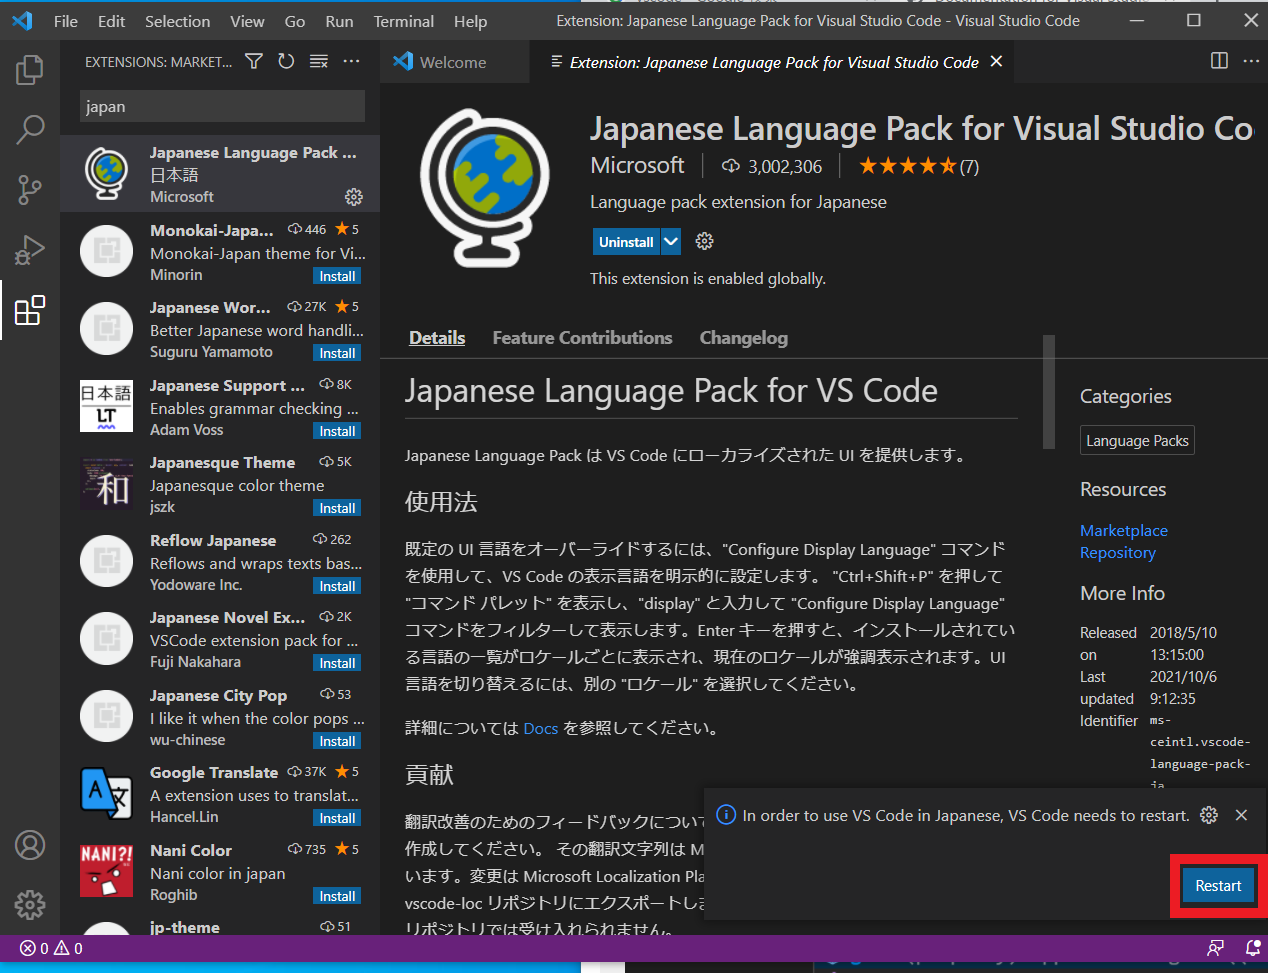
\includegraphics[width=10cm]{images/VSCodeExtension3.png}
    \caption{VSCodeのリスタート}
\end{figure}

\subsection{LaTeX WorkShopのインストール}

日本語パッケージをインストールした時と同様に四角形が4つあるアイコンをクリックしてください。(図28)
図29のオレンジ枠にある検索枠が表示されたら『LaTeX』と入力してください。
赤枠のような万年筆のアイコンをクリックしてください。
『LaTeX Workshop』が表示されます。
その後は、緑枠の位置にある『install』をクリックしてください。
以上でLaTeX Workshopのインストールは完了です。

\begin{figure}[H]
    \begin{minipage}[b]{0.45\linewidth}
        \centering
        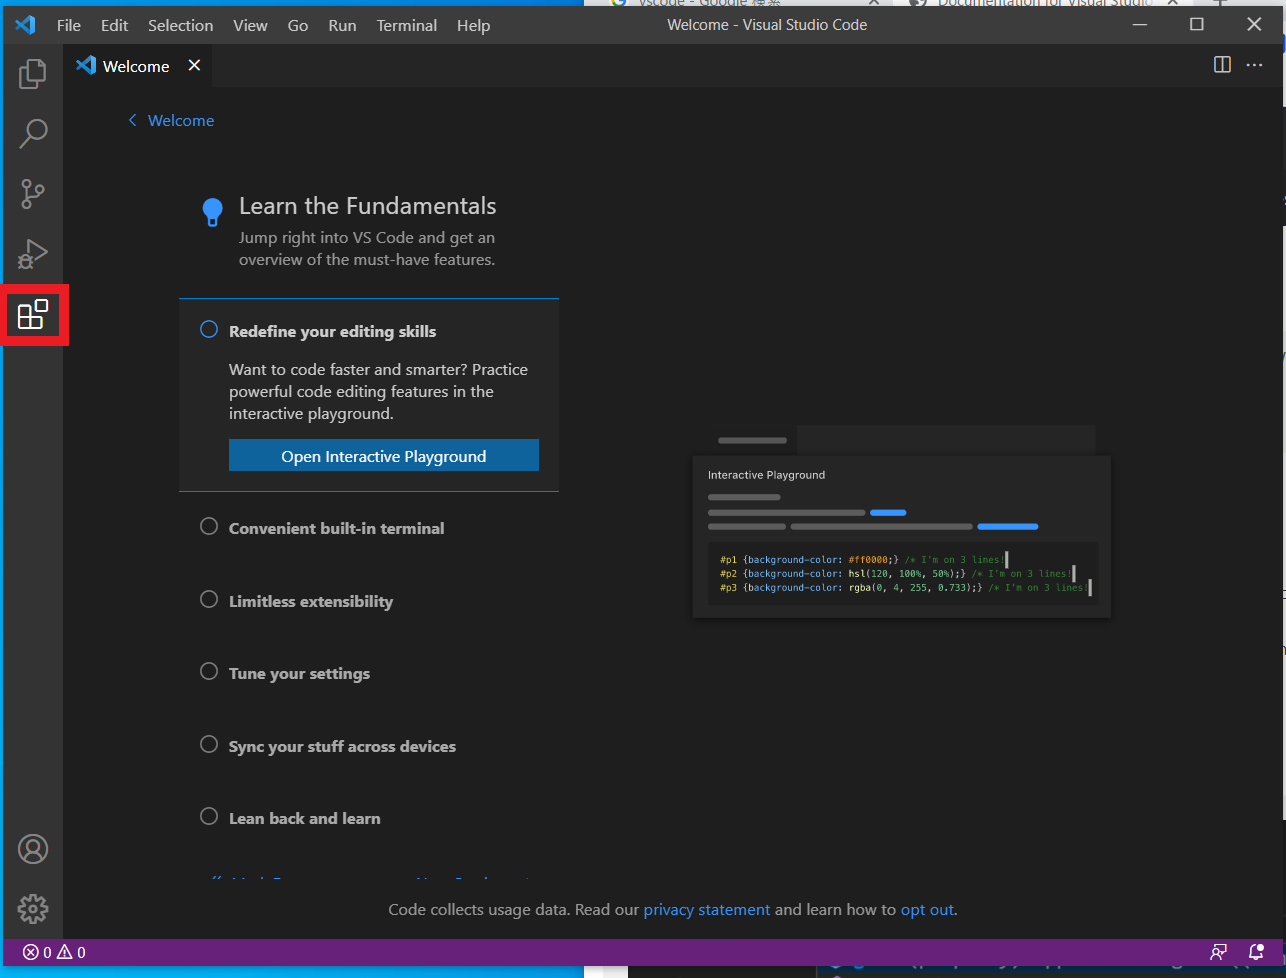
\includegraphics[width=5cm]{images/VSCodeExtension1.png}
        \caption{VSCode初期画面}
    \end{minipage}
    \begin{minipage}[b]{0.45\linewidth}
        \centering
        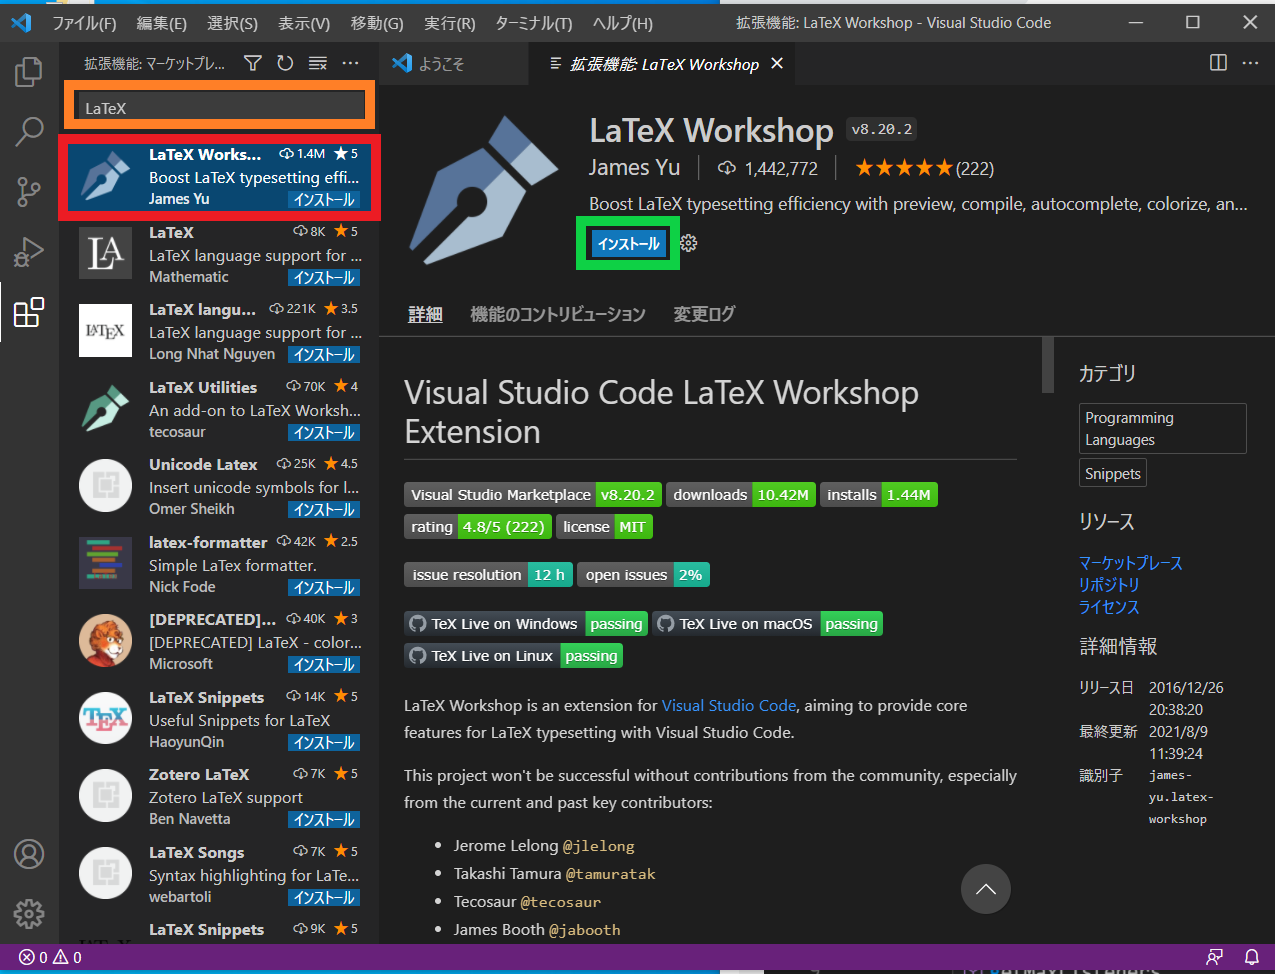
\includegraphics[width=5cm]{images/VSCodeExtension4.png}
        \caption{LaTeX Workshop}
    \end{minipage}
\end{figure}

\subsection{LaTeX Workshopの設定}

TeXファイルをビルドするためにLaTeX Workshopを設定していきます。
図30のオレンジ枠の『表示』をクリックすると、メニューが表示されるので、赤枠の『コマンドパレットを表示』をクリックしてください。
コマンドパレットが表示されたら、図31のようにオレンジ枠の検索枠に『settingj』と入力すると、関連メニューが表示されます。
メニューの中から赤枠の『基本設定:設定(JSON)を開く』をクリックしてください。

\begin{figure}[H]
    \begin{minipage}[b]{0.45\linewidth}
        \centering
        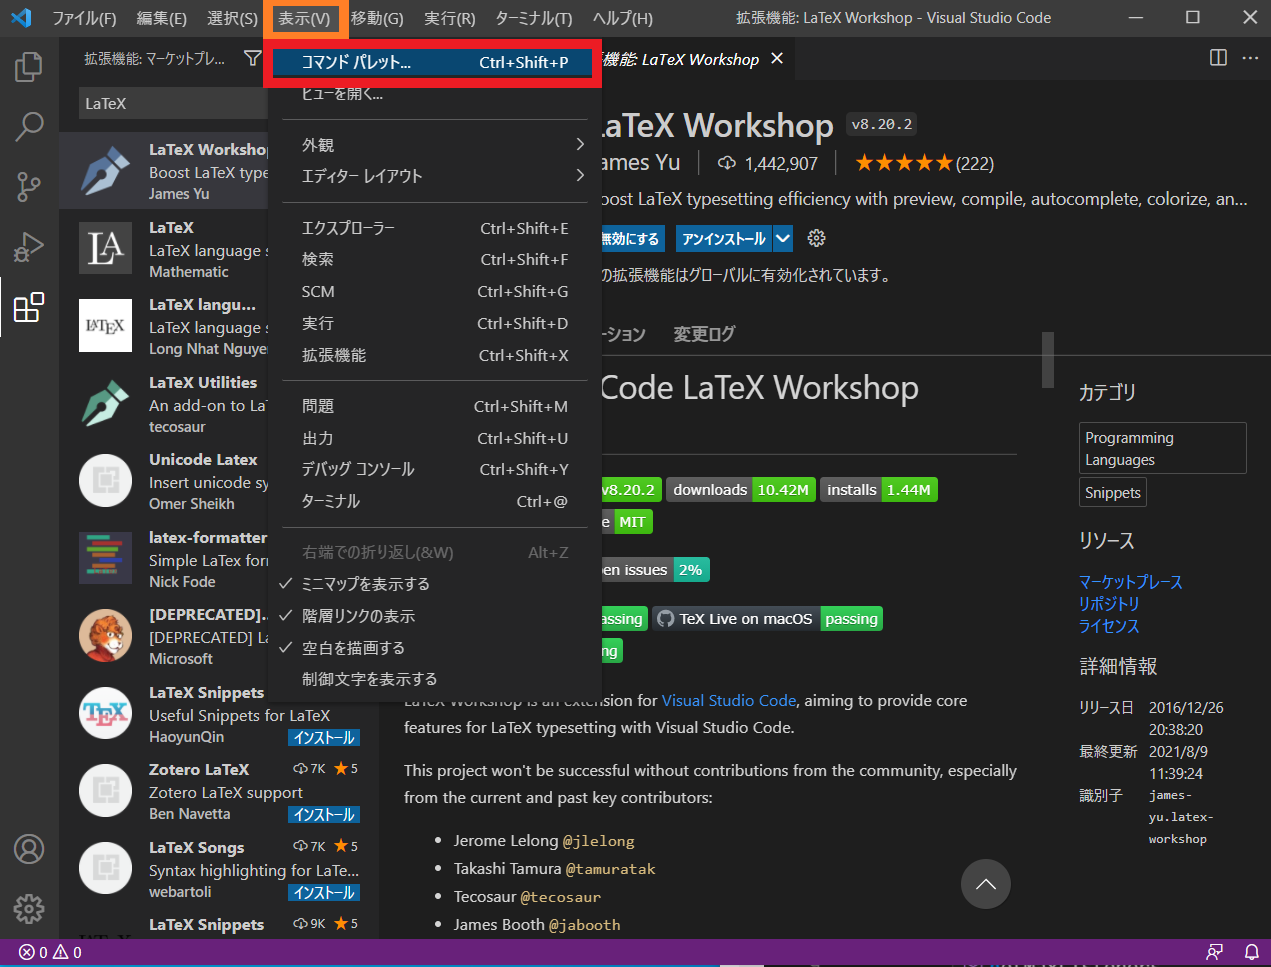
\includegraphics[width=5cm]{images/LaTeXWorkshop1.png}
        \caption{コマンドパレットの表示}
    \end{minipage}
    \begin{minipage}[b]{0.45\linewidth}
        \centering
        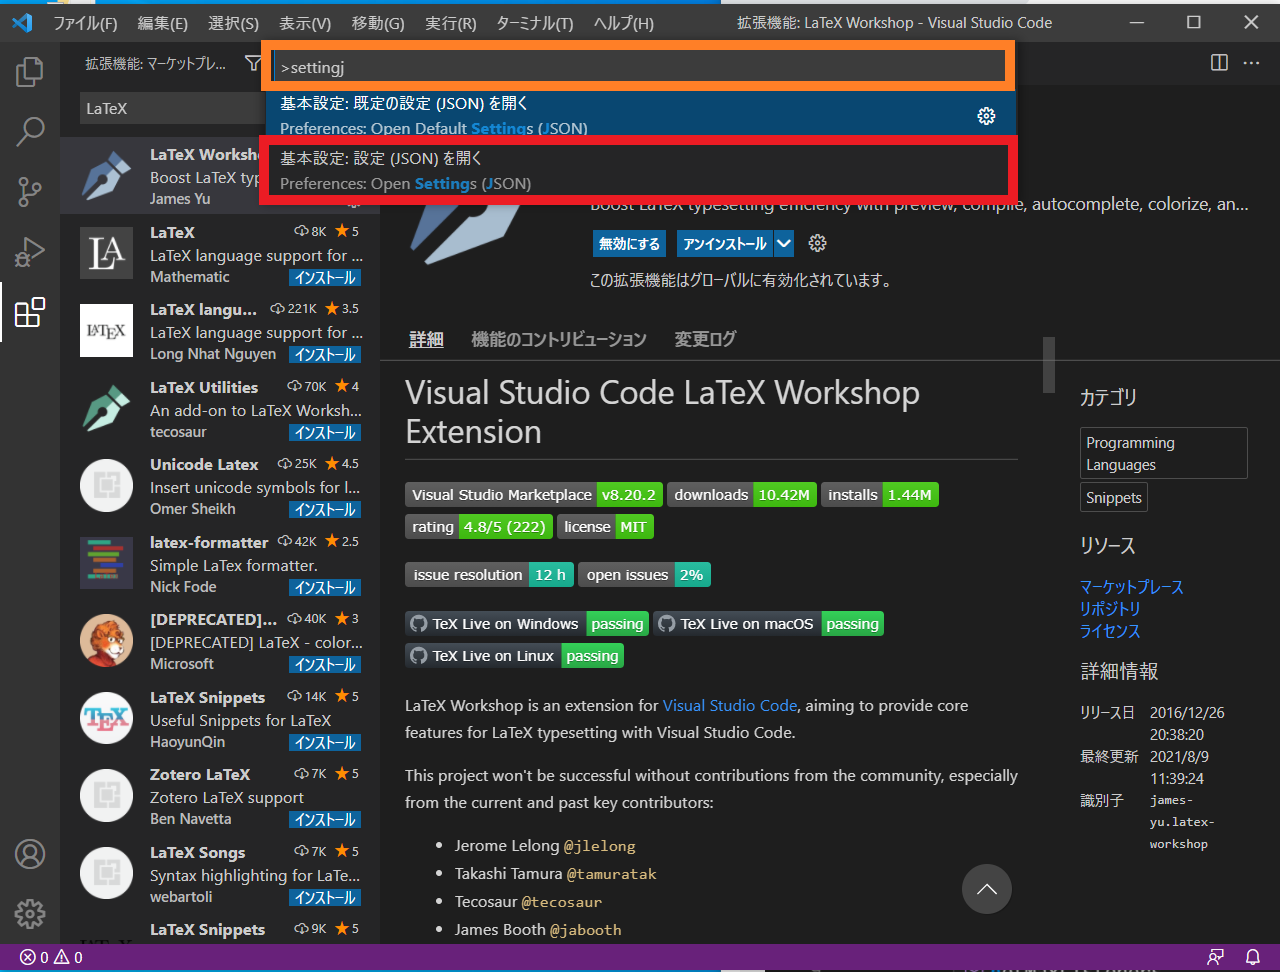
\includegraphics[width=5cm]{images/LaTeXWorkshop2.png}
        \caption{Setting.jsonの表示}
    \end{minipage}
\end{figure}

図30のような画面が表示されると思います。
内容を全て削除したのち、\href{https://github.com/CIT-NakamuraLab/thesis/blob/main/Windows/setting.json}{リンク先}のsetting.jsonをコピーして貼り付けてください。
リンク切れしている場合は、Listing1で記述されているsetting.jsonを利用してください。
以上で、LaTeXをWindows+VSCodeでビルドするための環境構築は終了です。

\begin{figure}[H]
    \begin{minipage}[b]{0.45\linewidth}
        \centering
        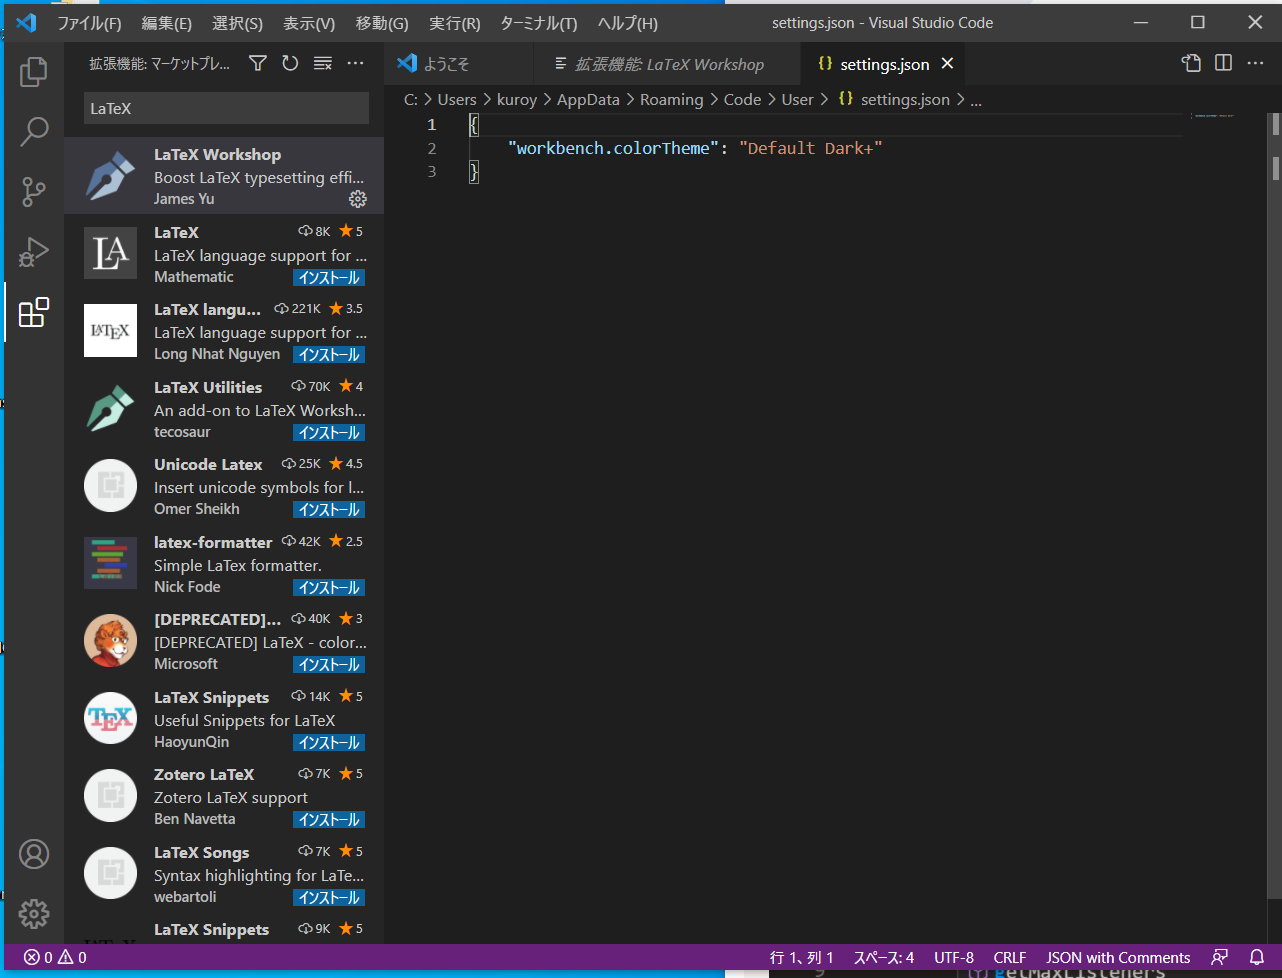
\includegraphics[width=5cm]{images/LaTeXWorkshop3.png}
        \caption{デフォルトのsetting.json}
    \end{minipage}
    \begin{minipage}[b]{0.45\linewidth}
        \centering
        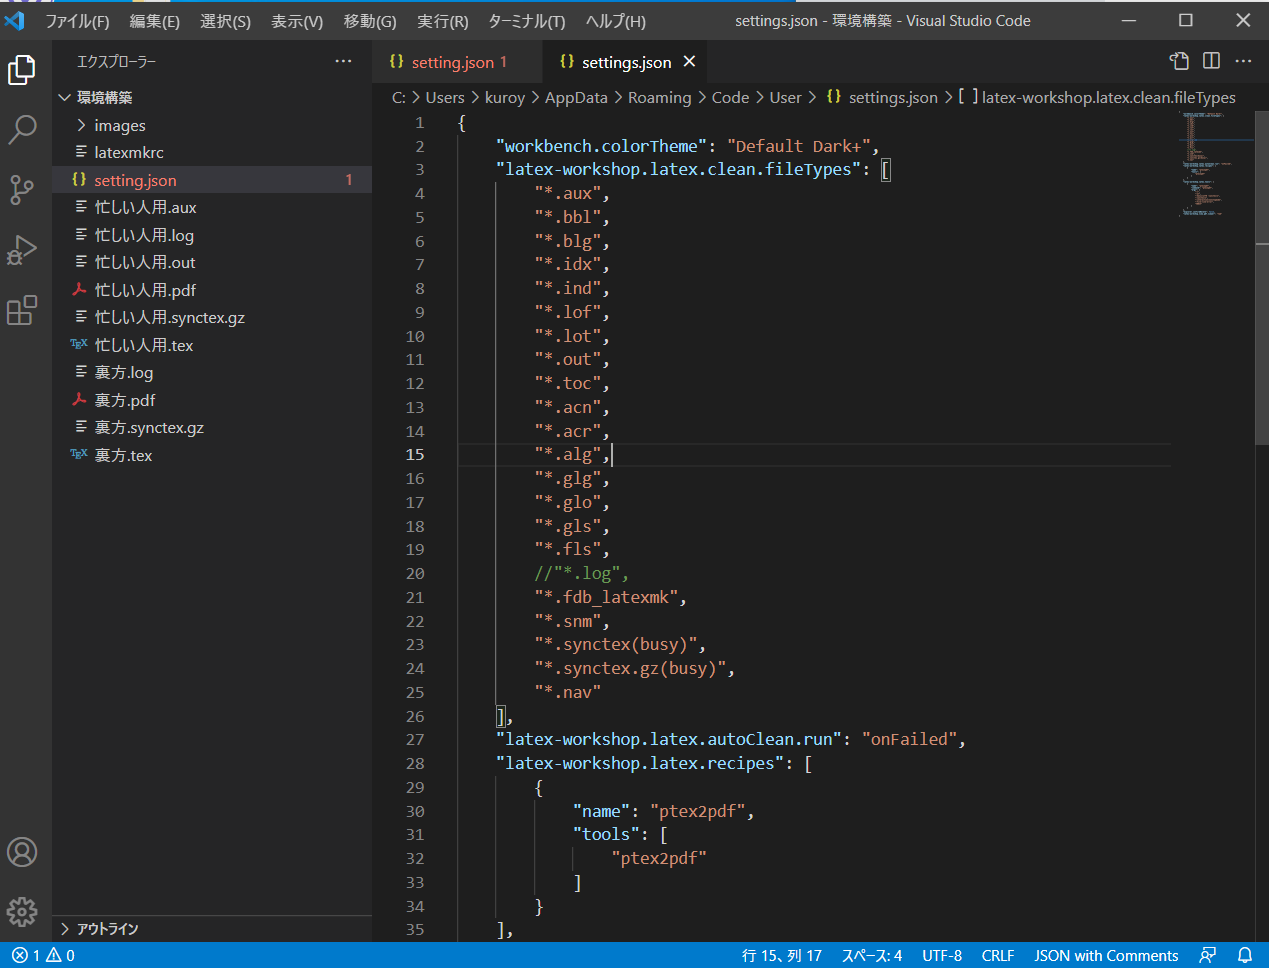
\includegraphics[width=5cm]{images/LaTeXWorkshop4.png}
        \caption{設定後のsetting.jsonの一部}
    \end{minipage}
\end{figure}

\lstinputlisting[caption=setting.json]{setting.json}

\section{おわりに}

LaTeXでソースコードを扱う場合別途の設定が必要になります。
その環境構築は別でおこないます。お待ちください。

\end{document}